% !TeX program = xelatex
% !TeX encoding = UTF-8
\documentclass{article}
\usepackage{ctex}
\usepackage{geometry}
\geometry{a4paper, left=3cm, right=3cm, top=2.5cm, bottom=2.5cm}

\usepackage{graphicx}
\usepackage{enumerate}
\usepackage{amsmath, amssymb, amsthm}
\usepackage{algorithm, algorithmic}
\floatname{algorithm}{算法}
\renewcommand{\algorithmicrequire}{\textbf{输入:}}
\renewcommand{\algorithmicensure}{\textbf{输出:}}

\usepackage{listings}
\usepackage{xcolor}
\usepackage{hyperref}
\hypersetup{colorlinks, citecolor=black, filecolor=black, linkcolor=black, urlcolor=black}
\usepackage{booktabs}
% 代码样式
\lstset{
    language=C++,
    keywordstyle=\color{blue},
    commentstyle=\color{green!50!black},
    stringstyle=\color{red},
    numbers=left,
    numberstyle=\tiny,
    basicstyle=\ttfamily\small,
    frame=single,
    breaklines=true,
    extendedchars=false
}

\title{第六次上机作业}
\author{学号：241830137\quad 姓名：朱子健}
\date{\today}

\begin{document}

\maketitle

\section{问题}
求 $f(x) = e^{x}$ 在区间 $[0,1]$ 上的$n$次最佳平方逼近多项式$\varphi(x)$:
\(
\varphi(x) = \sum_{k=0}^{n} a_k \varphi_k(x)
\)
\begin{itemize}
    \item $n = 5$, $\varphi_k(x) = x^k$;
    \item $n = 5$, $\varphi_k(x)$ 为第 $k$ 次 Legendre 多项式;
    \item $n = 10$, $\varphi_k(x) = x^k$;
    \item $n = 10$, $\varphi_k(x)$ 为第 $k$ 次 Legendre 多项式.
\end{itemize}

\section{算法原理与设计}
\subsection{算法原理}
\subsubsection{最佳平方逼近}
设 $f(x)\in C[a,b]$，$\Phi_{n+1}\subset C[a,b]$ 为区间 $[a,b]$ 上的一个线性无关函数系 $\{\phi_i(x)\}_{i=0}^{n}$ 张成的空间。若存在 $\phi^{*}(x)\in \Phi_{n+1}$ 使得
\[
\| f(x) - \phi^{*}(x) \|_{2}^{2} = \min_{\phi(x)\in \Phi_{n+1}} \| f(x) - \phi(x) \|_{2}^{2},
\]
则称 $\phi^{*}(x)$ 为 $f(x)$ 在区间 $[a,b]$ 上的\textbf{最佳平方逼近（函数）}。这里 $\|\cdot\|_{2}^{2}$ 是 $C[a,b]$ 上带权 $W(x)$ 的内积，即
\[
\| f(x) - \phi(x) \|_{2}^{2} = \bigl( f(x)-\phi(x), f(x)-\phi(x) \bigr) = \int_{a}^{b} \bigl[ f(x) - \phi(x) \bigr]^{2} W(x) \, \mathrm{d}x.
\]
设 $f(x)\in C[a,b]$，$\Phi_{n+1}=\operatorname{span}\{\phi_0(x),\phi_1(x),\dots,\phi_n(x)\}$ 为给定的线性无关函数系。在 $\Phi_{n+1}$ 中寻求 $f(x)$ 的最佳平方逼近函数
\[
\phi^*(x) = \sum_{j=0}^n c_j \phi_j(x),
\]
即求系数 $c_0,c_1,\dots,c_n$ 使误差平方积分
\[
\|f-\phi\|_2^2 = \int_a^b \bigl[ f(x) - \sum_{j=0}^n c_j \phi_j(x) \bigr]^2 W(x)\,dx
\]
达到最小。由极值必要条件 $\frac{\partial}{\partial c_i}=0$ 导出法方程组（讲义式 (3.4.5)）：
\[
\sum_{j=0}^n (\phi_j,\phi_i) c_j = (f,\phi_i), \quad i=0,1,\dots,n,
\]
其中内积定义为
\[
(\phi_j,\phi_i) = \int_a^b \phi_j(x)\phi_i(x) W(x)\,dx, \quad (f,\phi_i) = \int_a^b f(x)\phi_i(x) W(x)\,dx.
\]
写成矩阵形式为
\[
\begin{bmatrix}
(\phi_0,\phi_0) & (\phi_1,\phi_0) & \cdots & (\phi_n,\phi_0) \\
(\phi_0,\phi_1) & (\phi_1,\phi_1) & \cdots & (\phi_n,\phi_1) \\
\vdots & \vdots & \ddots & \vdots \\
(\phi_0,\phi_n) & (\phi_1,\phi_n) & \cdots & (\phi_n,\phi_n)
\end{bmatrix}
\begin{bmatrix}
c_0 \\ c_1 \\ \vdots \\ c_n
\end{bmatrix}
=
\begin{bmatrix}
(f,\phi_0) \\ (f,\phi_1) \\ \vdots \\ (f,\phi_n)
\end{bmatrix}.
\]
该方程组的系数矩阵为 Gram 矩阵，对称正定，当基函数线性无关时非奇异，故系数 $c_j$ 存在唯一。
\subsubsection{Legendre多项式}
当权函数 $W(x)=1$，区间为 $[-1,1]$ 时，可定义如下形式的正交多项式
\[
\begin{aligned}
P_n(x) &= \frac{1}{2^n n!} \frac{\mathrm{d}^n}{\mathrm{d}x^n} (x^2-1)^n, \quad n=1,2,\dots,\\
P_0(x) &= 1.
\end{aligned}
\]
我们称这样的正交多项式为 \textbf{Legendre 多项式}。
Legendre 多项式满足三项递推关系：
\[
(k+1)P_{k+1}(t) = (2k+1)t P_k(t) - k P_{k-1}(t), \quad k\ge 1.
\]
此外，由 Rodrigues 公式可导出导数恒等式：
\[
P_{k+1}'(t) - P_{k-1}'(t) = (2k+1) P_k(t). \tag{*}
\]
对 $I_k$ 应用一次分部积分：
\begin{align*}
I_k &= \int_{-1}^{1} e^{c t} P_k(t)\,dt 
     = \left[ \frac{1}{c} e^{c t} P_k(t) \right]_{-1}^{1} - \frac{1}{c} \int_{-1}^{1} e^{c t} P_k'(t)\,dt \\
    &= \frac{1}{c}\bigl( e^{c} - (-1)^k e^{-c} \bigr) - \frac{1}{c} \int_{-1}^{1} e^{c t} P_k'(t)\,dt. \tag{1}
\end{align*}
利用恒等式 $(*)$ 替换 $P_k'(t)$：
\[
P_k'(t) = \frac{1}{2k+1}\bigl( P_{k+1}'(t) - P_{k-1}'(t) \bigr).
\]
代入 (1) 中的积分项：
\[
\int_{-1}^{1} e^{c t} P_k'(t)\,dt 
= \frac{1}{2k+1} \left( \int_{-1}^{1} e^{c t} P_{k+1}'(t)\,dt - \int_{-1}^{1} e^{c t} P_{k-1}'(t)\,dt \right).
\]
对右侧两积分再次分部积分（反向操作）：
\begin{align*}
\int_{-1}^{1} e^{c t} P_{m}'(t)\,dt 
&= \bigl[ e^{c t} P_m(t) \bigr]_{-1}^{1} - c \int_{-1}^{1} e^{c t} P_m(t)\,dt \\
&= \bigl( e^{c} - (-1)^m e^{-c} \bigr) - c I_m.
\end{align*}
将 $m=k+1$ 与 $m=k-1$ 代入，整理后得到关于 $I_{k+1}, I_k, I_{k-1}$ 的递推式：
\[
I_{k+1} = \frac{2k+1}{c} I_k - I_{k-1} - \frac{2k+1}{c}\bigl( e^{c} - (-1)^k e^{-c} \bigr). \tag{2}
\]
代入 $c = 1/2$，即得数值递推公式：
\[
\boxed{
I_{k+1} = 2(2k+1) I_k - I_{k-1} - 2(2k+1)\bigl( e^{1/2} - (-1)^k e^{-1/2} \bigr), \quad k=1,2,\dots
}
\]

\subsubsection{算法设计}
\begin{algorithm}[H]
\caption{求函数$e^{x}$的最佳平方逼近多项式，基函数为$\varphi_{k}(x) = x^{k}$}
\begin{algorithmic}[1]
    \REQUIRE 逼近次数 $n$
    \ENSURE 展开系数 $\{a_k\}_{k=0}^{n}$
    \STATE \textbf{Step 1:} 计算右端向量 $\mathbf{b} = (b_0, b_1, \dots, b_n)^T$
    \STATE \quad $b_0 \gets e - 1$
    \FOR{$j = 1$ \TO $n$}
        \STATE $b_j \gets e - j \cdot b_{j-1}$ \COMMENT{分部积分递推}
    \ENDFOR
    \STATE \textbf{Step 2:} 构造法方程矩阵 $G \in \mathbb{R}^{(n+1)\times (n+1)}$
    \FOR{$i = 0$ \TO $n$}
        \FOR{$j = 0$ \TO $n$}
            \STATE $G_{ij} \gets \dfrac{1}{i+j+1}$ \COMMENT{Hilbert 矩阵}
        \ENDFOR
    \ENDFOR

    \STATE \textbf{Step 3:} 解线性方程组 $G \mathbf{a} = \mathbf{b}$，得系数向量 $\mathbf{a}$
    \STATE \textbf{Step 4:} 输出 $\mathbf{a} = (a_0, a_1, \dots, a_n)^T$

\end{algorithmic}
\end{algorithm}

\begin{algorithm}[H]
\caption{求函数$e^{x}$的最佳平方逼近多项式，基函数为Legendre多项式}
\begin{algorithmic}[1]
    \REQUIRE 逼近次数 $n$
    \ENSURE 展开系数 $\{a_k\}_{k=0}^{n}$
    \STATE \textbf{Step 1:} 计算初值
    \STATE \quad $I_0 \gets 2(e^{0.5} - e^{-0.5})$
    \STATE \quad $I_1 \gets 6 e^{0.5} + 2 e^{-0.5}$

    \STATE \textbf{Step 2:} 正向递推 $I_2, I_3, \dots, I_n$
    \FOR{$k = 1$ \TO $n-1$}
        \STATE $I_{k+1} \gets 2(2k+1) I_k - I_{k-1} - 2(2k+1)\bigl( e^{0.5} - (-1)^k e^{-0.5} \bigr)$
    \ENDFOR

    \STATE \textbf{Step 3:} 计算系数 $a_k$
    \FOR{$k = 0$ \TO $n$}
        \STATE $a_k \gets \dfrac{2k+1}{2} \cdot e^{0.5} \cdot I_k$
    \ENDFOR

    \STATE \textbf{Step 4:} 输出 $\{a_k\}_{k=0}^{n}$
\end{algorithmic}
\end{algorithm}
\section{结果分析}
\subsection{数值计算结果}
利用分部积分递推分别求出幂基法方程右端项 $b_j = \int_0^1 e^x x^j\,dx$ 以及 Legendre 基积分 $I_k = \int_{-1}^1 e^{t/2} P_k(t)\,dt$，进而得到两组最佳平方逼近多项式的展开系数。表~\ref{tab:coeff_power} 和表~\ref{tab:coeff_legendre} 分别列出 $n=5$ 和 $n=10$ 时的系数（保留 6 位有效数字）。

\begin{table}[H]
\centering
\caption{幂基最佳平方逼近系数 $a_k$（$f(x)=e^x$ 在 $[0,1]$ 上）}
\label{tab:coeff_power}
\begin{tabular}{c|cccccc}
\toprule
$n$ & $a_0$ & $a_1$ & $a_2$ & $a_3$ & $a_4$ & $a_5$ \\
\midrule
5  & 1.000027 & 0.998866 & 0.509920 & 0.140342 & 0.069395 & -0.006249 \\
10 & 1.000000 & 1.000000 & 0.500000 & 0.166667 & 0.041667 & 0.008333 \\
\bottomrule
\multicolumn{7}{c}{}\\
\toprule
$n$ & $a_6$ & $a_7$ & $a_8$ & $a_9$ & $a_{10}$ \\
\midrule
10 & 0.001389 & 0.000198 & 0.000025 & 0.000003 & 0.000000 \\
\bottomrule
\end{tabular}
\end{table}

\begin{table}[H]
\centering
\caption{Legendre 基最佳平方逼近系数 $c_k$（$f(x)=e^x$ 在 $[0,1]$ 上）}
\label{tab:coeff_legendre}
\begin{tabular}{c|cccccc}
\toprule
$n$ & $c_0$ & $c_1$ & $c_2$ & $c_3$ & $c_4$ & $c_5$ \\
\midrule
5  & 1.718282 & 0.845155 & 0.139864 & 0.013794 & 0.000930 & 0.000046 \\
10 & 1.718282 & 0.845155 & 0.139864 & 0.013794 & 0.000930 & 0.000046 \\
\bottomrule
\multicolumn{7}{c}{}\\
\toprule
$n$ & $c_6$ & $c_7$ & $c_8$ & $c_9$ & $c_{10}$ \\
\midrule
10 & 1.75e-6 & 5.3e-8 & 1.3e-9 & 2.7e-11 & 4.7e-13 \\
\bottomrule
\end{tabular}
\end{table}

\begin{figure}[H]
\centering

\includegraphics[width=0.9\textwidth]{Figure_1.png}
\caption{$n=5$ 时的逼近曲线（左）与绝对误差（右）}
\label{fig:n5}
\end{figure}

\begin{figure}[H]
\centering
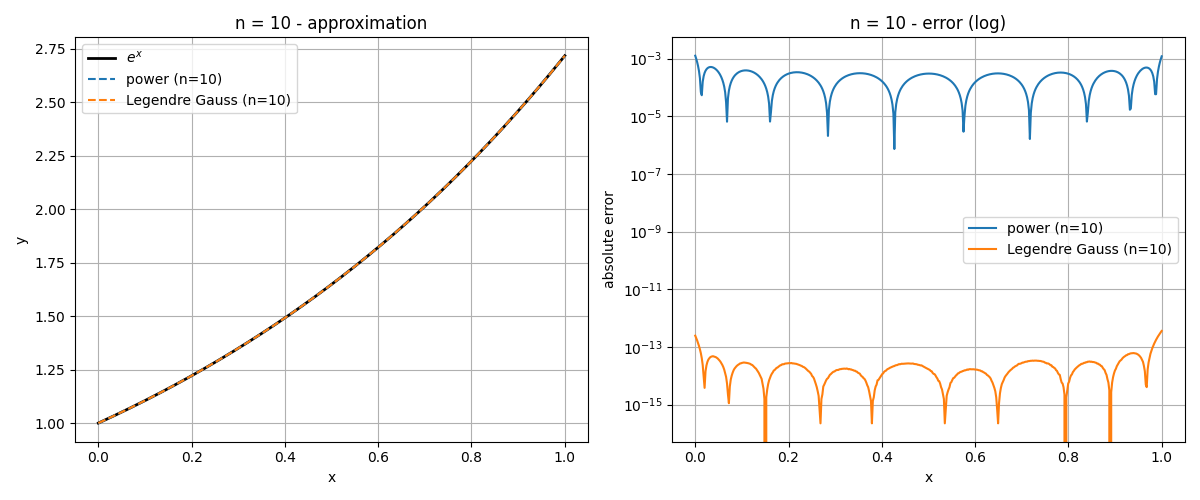
\includegraphics[width=0.9\textwidth]{Figure_2.png}
\caption{$n=10$ 时的逼近曲线（左）与绝对误差（右）}
\label{fig:n6}
\end{figure}

\subsection{数值计算结果分析}
幂基对应的法方程矩阵为 Hilbert 矩阵 $\mathbf{H}_{n+1}$，其元素 $H_{ij}=1/(i+j+1)$。随着 $n$ 增大，系数出现了偏差，这正是病态矩阵放大舍入误差的结果。
Legendre 多项式在 $[-1,1]$ 上关于权 $W(x)\equiv1$ 正交，法方程矩阵为对角阵，无需解方程组，系数由内积直接计算。因此不存在病态问题，系数精度仅受积分计算精度控制。
\section{附录: Python 源代码实现}
\begin{lstlisting}[language=Python]
import numpy as np
import matplotlib.pyplot as plt
from scipy.special import eval_legendre
from numpy.polynomial.legendre import leggauss

def f(x):
    return np.exp(x)

def power_basis_coeffs(n, high_precision=False):
    if high_precision:
        from decimal import Decimal, getcontext
        getcontext().prec = 50
        e = Decimal(np.e).exp()
        b = [Decimal(0)] * (n + 1)
        b[0] = e - Decimal(1)
        for j in range(1, n + 1):
            b[j] = e - Decimal(j) * b[j-1]
        H = np.zeros((n + 1, n + 1), dtype=object)
        for i in range(n + 1):
            for j in range(n + 1):
                H[i, j] = Decimal(1) / Decimal(i + j + 1)
        a = np.linalg.solve(H.astype(float), np.array(b, dtype=float))
        return a
    else:
        b = np.zeros(n + 1)
        b[0] = np.e - 1
        for j in range(1, n + 1):
            b[j] = np.e - j * b[j-1]
        H = np.fromfunction(lambda i, j: 1.0 / (i + j + 1), (n + 1, n + 1))
        a = np.linalg.solve(H, b)
        return a

def power_approx(x, coeffs):
    return np.polyval(coeffs[::-1], x)

def legendre_coeffs(n, method='gauss', N_gauss=50):
    e_half = np.exp(0.5)
    if method == 'gauss':
        t, w = leggauss(N_gauss)
        ft = e_half * np.exp(t / 2.0)
        coeffs = np.zeros(n + 1)
        for k in range(n + 1):
            Pk = eval_legendre(k, t)
            integral = np.sum(w * ft * Pk)
            coeffs[k] = (2 * k + 1) / 2.0 * integral
        return coeffs
    elif method == 'recur':
        e_n = np.exp(-0.5)
        I = np.zeros(n + 1)
        I[0] = 2.0 * (e_half - e_n)
        if n >= 1:
            I[1] = 6.0 * e_half + 2.0 * e_n
        for k in range(1, n):
            term = e_half - ((-1) ** k) * e_n
            I[k+1] = 2.0 * (2 * k + 1) * I[k] - I[k-1] - 2.0 * (2 * k + 1) * term
        coeffs = (2.0 * np.arange(n + 1) + 1) / 2.0 * e_half * I
        return coeffs

def legendre_approx(x, coeffs):
    t = 2.0 * x - 1.0
    n = len(coeffs) - 1
    val = np.zeros_like(x)
    for k in range(n + 1):
        val += coeffs[k] * eval_legendre(k, t)
    return val

def compute_errors(x_test, y_true, y_approx):
    abs_err = np.abs(y_true - y_approx)
    max_err = np.max(abs_err)
    l2_err = np.sqrt(np.trapezoid((y_true - y_approx)**2, x_test))
    return max_err, l2_err

def plot_results(x_plot, y_true, approx_dict, title):
    plt.figure(figsize=(12, 5))
    plt.subplot(1, 2, 1)
    plt.plot(x_plot, y_true, 'k-', linewidth=2, label='$e^x$')
    for label, y_app in approx_dict.items():
        plt.plot(x_plot, y_app, '--', label=label)
    plt.xlabel('x')
    plt.ylabel('y')
    plt.title(title + ' - approximation')
    plt.legend()
    plt.grid(True)
    plt.subplot(1, 2, 2)
    for label, y_app in approx_dict.items():
        err = np.abs(y_true - y_app)
        plt.semilogy(x_plot, err, label=label)
    plt.xlabel('x')
    plt.ylabel('absolute error')
    plt.title(title + ' - error (log)')
    plt.legend()
    plt.grid(True)
    plt.tight_layout()
    plt.savefig(f'figure_n{title.split("=")[1].strip()}.pdf', bbox_inches='tight')
    plt.show()

if __name__ == "__main__":
    n_list = [5, 10]
    x_plot = np.linspace(0, 1, 500)
    y_true = f(x_plot)
    for n in n_list:
        print(f"\n{'='*60}\n n = {n}\n{'='*60}")
        a_pow = power_basis_coeffs(n, high_precision=False)
        print(f"\npower coeffs (n={n}):")
        for k, ak in enumerate(a_pow):
            print(f"  a_{k} = {ak:15.10f}")
        y_pow = power_approx(x_plot, a_pow)
        max_err_pow, l2_err_pow = compute_errors(x_plot, y_true, y_pow)
        print(f"max error: {max_err_pow:.4e}, L2 error: {l2_err_pow:.4e}")
        if n == 10:
            a_pow_hp = power_basis_coeffs(n, high_precision=True)
            print("\npower coeffs (high precision, n=10):")
            for k, ak in enumerate(a_pow_hp):
                print(f"  a_{k} = {ak:15.10f}")
        c_leg_gauss = legendre_coeffs(n, method='gauss')
        print(f"\nLegendre coeffs (Gauss, n={n}):")
        for k, ck in enumerate(c_leg_gauss):
            print(f"  c_{k} = {ck:15.10f}")
        y_leg_gauss = legendre_approx(x_plot, c_leg_gauss)
        max_err_leg, l2_err_leg = compute_errors(x_plot, y_true, y_leg_gauss)
        print(f"max error: {max_err_leg:.4e}, L2 error: {l2_err_leg:.4e}")
        c_leg_recur = legendre_coeffs(n, method='recur')
        print(f"\nLegendre coeffs (recur, n={n}):")
        for k, ck in enumerate(c_leg_recur):
            print(f"  c_{k} = {ck:15.10f}")
        y_leg_recur = legendre_approx(x_plot, c_leg_recur)
        max_err_leg2, l2_err_leg2 = compute_errors(x_plot, y_true, y_leg_recur)
        print(f"max error: {max_err_leg2:.4e}, L2 error: {l2_err_leg2:.4e}")
        approx_dict = {
            f'power (n={n})': y_pow,
            f'Legendre Gauss (n={n})': y_leg_gauss,
        }
        plot_results(x_plot, y_true, approx_dict, f'n = {n}')
    print("\n" + "="*60)
    print("Hilbert matrix condition numbers (power basis):")
    for n in [5, 10]:
        H = np.fromfunction(lambda i, j: 1.0/(i+j+1), (n+1, n+1))
        print(f"n={n}: cond(H) = {np.linalg.cond(H):.2e}")
    print("Legendre basis condition number = 1")
\end{lstlisting}

\end{document}